\documentclass{article}
\usepackage{lipsum}
\usepackage{amsmath}
\usepackage{hyperref}
\usepackage{xcolor}
\usepackage{amsfonts}
\usepackage{graphicx}

\usepackage{enumitem}
\setlist[enumerate]{itemsep=-1mm}


\topmargin=-0.65in    % Make letterhead sftart about 1 inch from top of page
\textheight=9.10in    % text height can be bigger for a longer letter
\oddsidemargin=-0.1in % leftmargin is 1 inch
\textwidth=6.7in   % textwidth of 6.5in leaves 1 inch for right margin

% some shortcuts
\newcommand{\ea}{\textit{et al. }} 
\newcommand{\ttt}[1]{\texttt{#1}}
\newcommand{\eg}{\textit{e.g. }} 
\newcommand{\ie}{\textit{i.e. }} 
\newcommand{\la}{\langle}
\newcommand{\ra}{\rangle}
\newcommand{\cg}{\color{gray}}
\newcommand{\fs}{\footnotesize}
\setlength{\parindent}{0mm}


%%%%%%%%%%%%%%%%%%%%%%%%%%%%%%%%%%%%%%%%%%%%%%%%%%%%%%%%%%%%%%%%%%%%%%%%
%%%%%%%%%%%%%%%%%%%%%%%%%%%%%%%%%%%%%%%%%%%%%%%%%%%%%%%%%%%%%%%%%%%%%%%%
%%%%%%%%%%%%%%%%%%%%%%%%%%%%%%%%%%%%%%%%%%%%%%%%%%%%%%%%%%%%%%%%%%%%%%%%
%%%%%%%%%%%%%%%%%%%%%%%%%%%%%%%%%%%%%%%%%%%%%%%%%%%%%%%%%%%%%%%%%%%%%%%%
\begin{document}


%%%%%%%%%%%%%%%%%%%%%%%%%%%%%%%%%%%%%%%%%%%%%%%%%%%%%%%%%%%%%%%%%%%%%%%%
%%%%%%%%%%%%%%%%%%%%%%%%%%%%%%% OUTLINE %%%%%%%%%%%%%%%%%%%%%%%%%%%%%%%%
%%%%%%%%%%%%%%%%%%%%%%%%%%%%%%%%%%%%%%%%%%%%%%%%%%%%%%%%%%%%%%%%%%%%%%%%
\title{\bf Filter Design Cheatsheet}
\maketitle

\section{FIR Filter Design}
This cheatsheet is compiled from book Digital Signal Processing with MATLAB by Ingle \& Proakis. Page references are given as \#PageNo

\paragraph{Problem Statement}
Design a lowpass filter that has a passband $[0,\omega_p]$ with tolerance $\delta_1$ (or $R_p$ in dB) and a stopband $[\omega_s, \pi]$ with tolerance $\delta_2$ (or $A_s$ in dB) \---- see Figure \ref{fig:design}b,c.

In FIR we focus on linear-phase filters:
\begin{equation}
H(e^{j\omega})=H_r(\omega)e^{j(\beta-\alpha\omega)}
\end{equation}

where $\alpha$ is \textit{constant group delay} and $H_r$ is the amplitude. The impulse response of linear-phase filters is symmetric or antisymmetric about $alpha$, therefore $\alpha=\frac{M-1}{2}$ and $h(n)=h(M-1-n)$ where $M$ is the filter length. A central goal in FIR filter design is to keep $M$ minimal. Based on whether the filter is symmetric or anti-symmetric, and whether $M$ is odd or even, there are four types of filters well-accepted in the literature. Each of these filters has a different usage.:

\begin{table}[h]
\centering
\begin{tabular}{|l|l|l|l|l|} \hline
 & M & symm/anti-symm  & $\beta$ & usage \\ \hline
\textbf{Type I} & odd & symm & 0 & any\\
\textbf{Type I} & even & anti-symm & 0 & lowpass only (not highpass or bandstop (see \#233)) \\
\textbf{Type I} & odd & symm & $\pi/2$ & digital Hilbert transformers and differentiators (to take derivative)\\
\textbf{Type I} & even & anti-symm & $\pi/2$ & digital Hilbert transformers and differentiators (to take derivative)\\ \hline
\end{tabular}
\caption{Filter types}
\label{tab:types}
\end{table}

\subsection{Design approaches}
\begin{enumerate}
\item Windowing an ideal LP filter
\item Designing directly in Frequency Domain
\item Optimal equiripple design
\end{enumerate}

The first two are intuitive but not optimal. The third has a more sophisticated theory but is optimal. Optimality here means minimal $M$ for given design specs (\ie desired $\omega_p, \omega_s, R_p, A_s$ values).

\subsubsection{Windowing an ideal lowpass filter}
An ideal lowpass (LP) filter (see Fig. \ref{fig:design}a) must be infinite. To make it FIR we must truncate the ideal filter, which will introduce ripples around cutoff frequency (see Fig. \ref{fig:design}b) due to Gibbs phenomenon (see \#245 onwards). The truncation is done by windowing, \ie multiplication (or conv in freq domain) with a windowing function. The goal  is to find the windowing function that meets the design specs with minimal $M$. The simplest and worse-performing windowing fn is boxcar. More sophisticate ones are triangular, Hanning, Hamming and Blackman. Hamming is typically used. See \#251 for comparison among windows.

\subsubsection{Designing directly in Frequency Domain}
We manually design a sequence in frequency domain such as $H(k) = \{1,1,1,1,0,0,0,0,0,0,0\}$ (number of 1's is proportional to $\omega_c$). This would be the freq response of the ideal filter. To minimize ripples, we manually introduce a slope such as $H(k) = \{1,1,1,T_1,T_2,0,0,0,0\}$. We decide the number of $T_i$ values, then the goal is to find the optimal $T_i$ values. See \#264 onwards.

\subsubsection{Optimal Equiriple Design}
It turns out that the optimal design is reached by distributing the error around ripples uniformly (in contrary to having an increasing error nearer the band edges). This can be performed with by solving what is called a \textit{minimax problem} (see \#278 onwards). This requires a polynomial approximation which is performed via the Parks-McClellan algorithm (\#284). 

All these can be done very simply in MATLAB through the \ttt{remez} function. The overall design is as follows:
\begin{enumerate}
\item Decide specs: $\omega_p, \omega_s, R_p, A_s$
\item Guess an initial filter length $\hat{M}$ (see code and 7.48 in \#284)
\item Run \ttt{remez}
\item check $A_s$, if OK stop, if not, increase $\hat{M}$ and repeat until desired $A_s$ reached. Bear in mind that the restrictions on $M$ based on the filter usage (see Table \ref{tab:types}) still apply and therefore $M$ should be incremented carefully (\ie maintain an either odd or even value).
\end{enumerate}


Exemlar piece of code: 

\begin{figure}
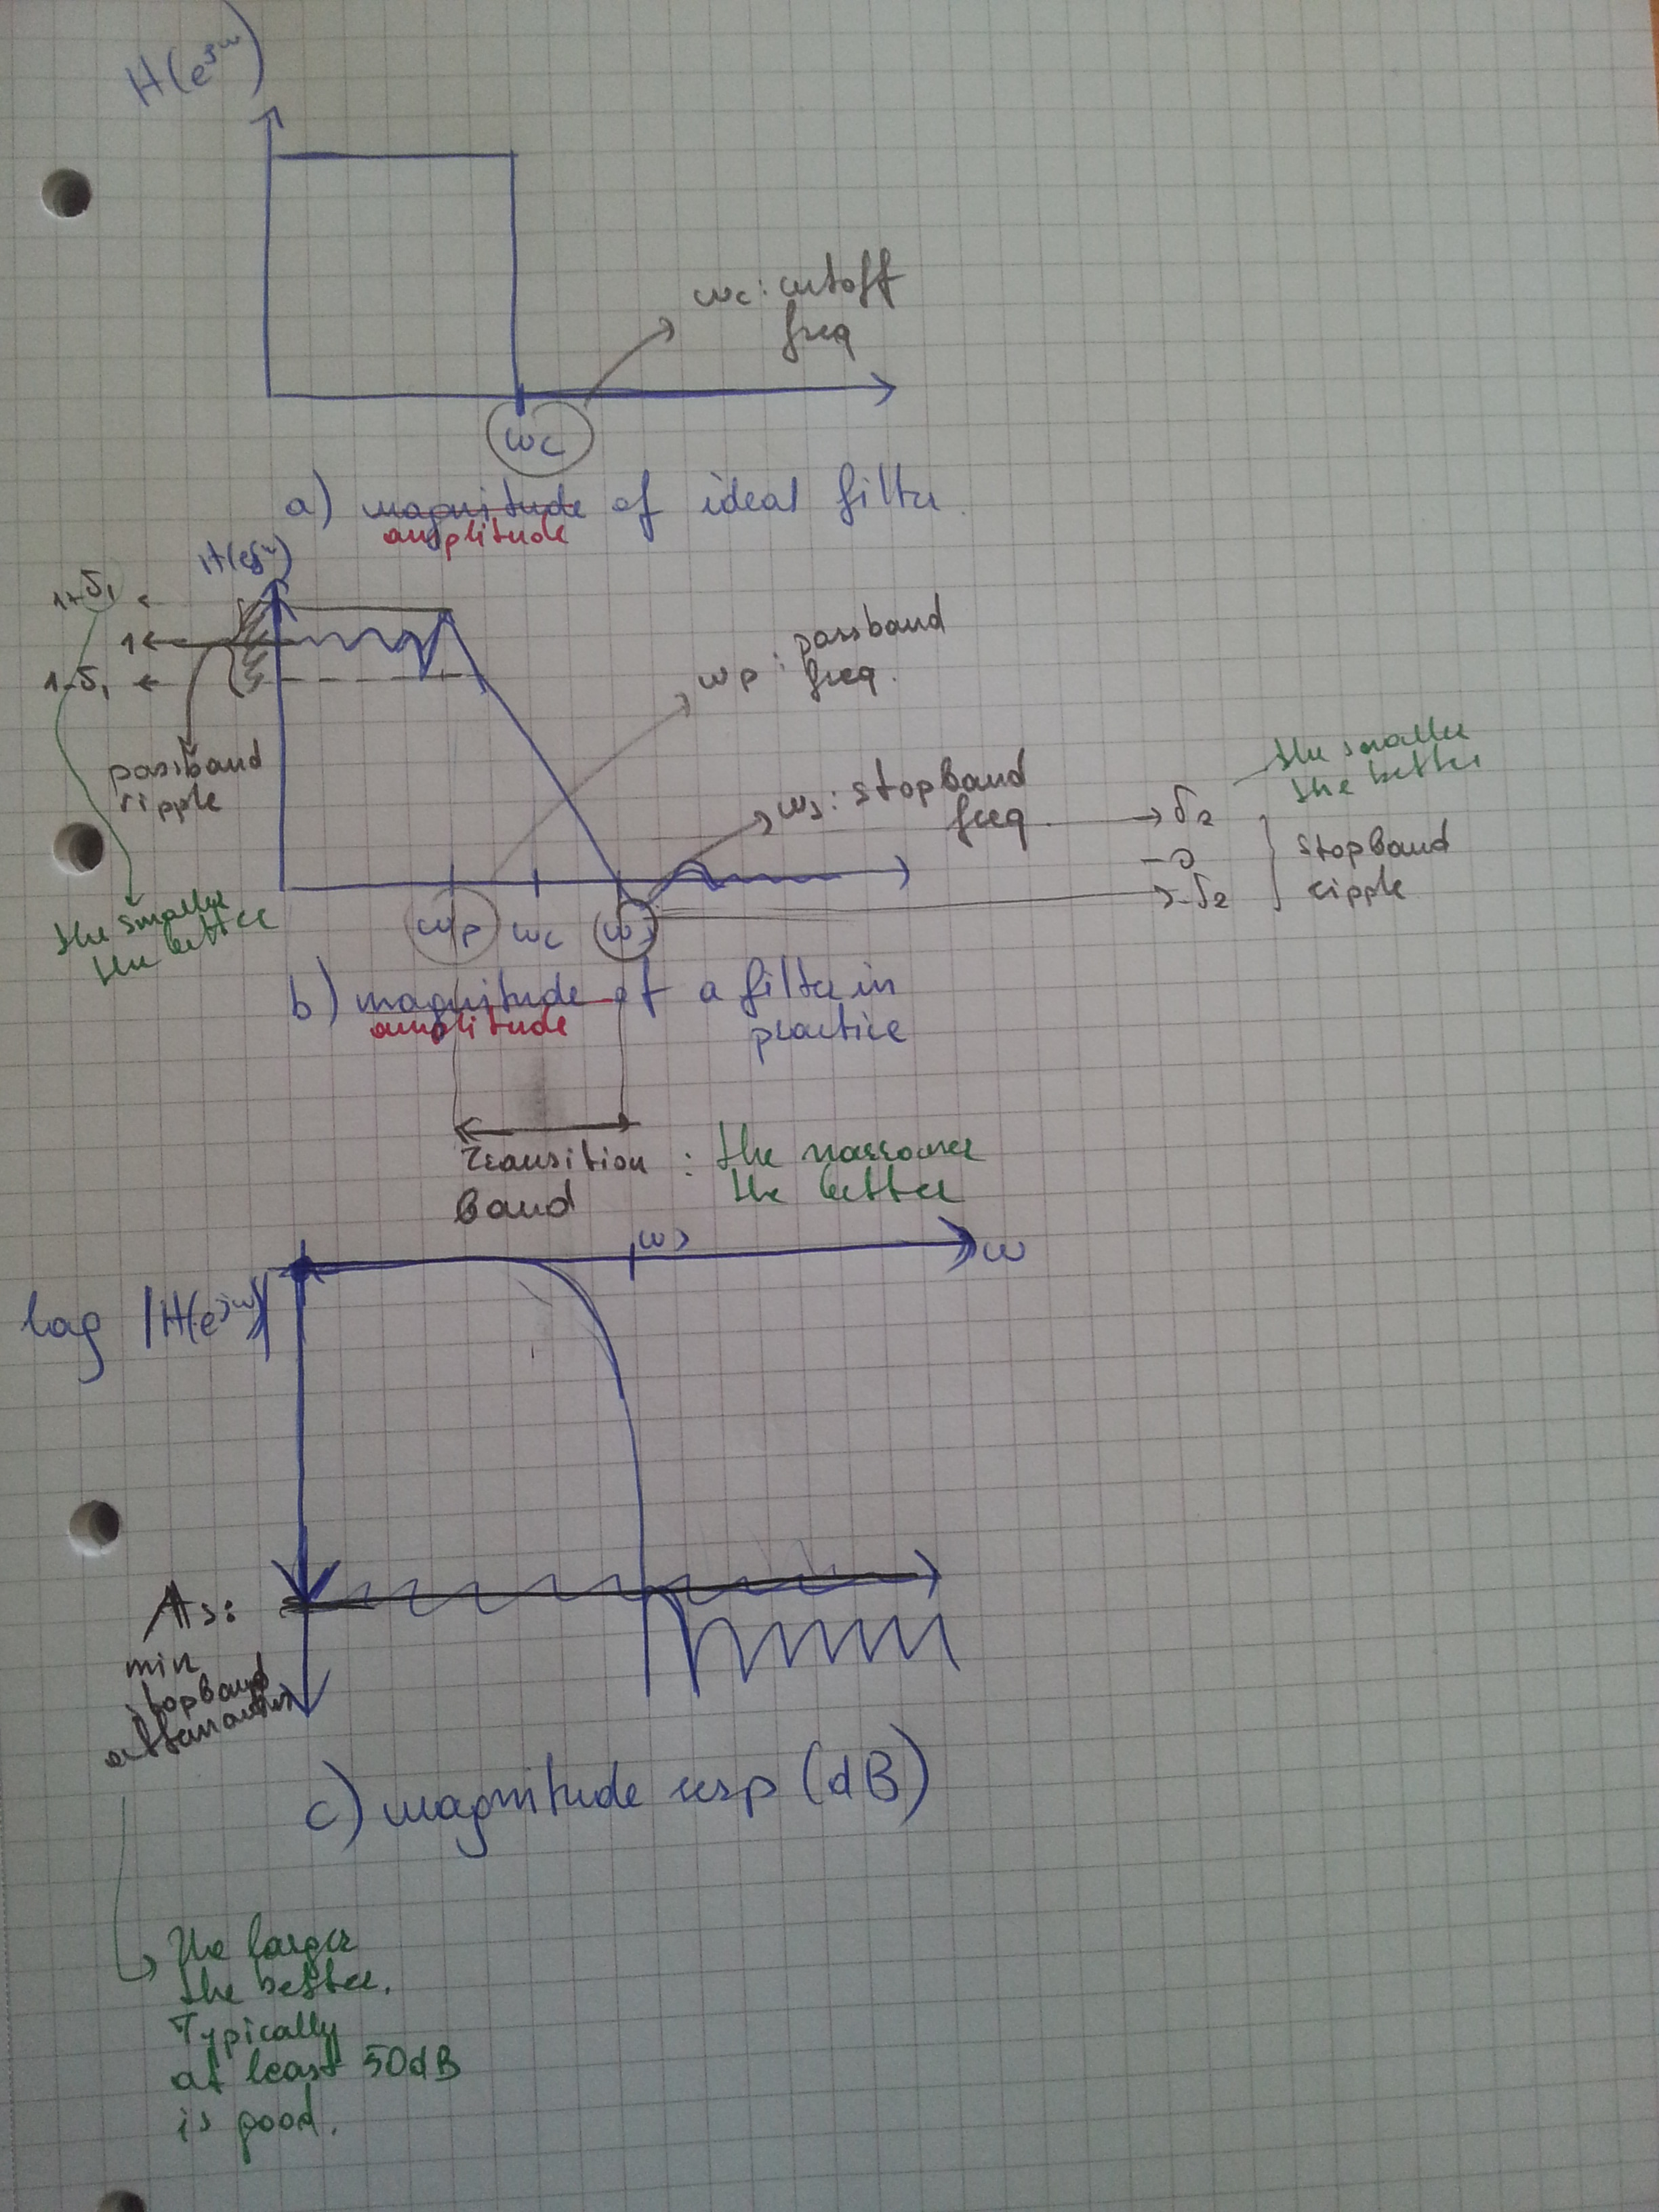
\includegraphics[scale=0.20]{fig/fir_design.jpg}
\label{fig:design}
\end{figure}

% https://www.youtube.com/watch?v=VXwXkME9uWU&list=PLMn2aW3wpAtOqo0g0OnHndXB1LnYBeMaX&index=1
\end{document}


